% ============================================================================
% Environmental Provisions in Chinese PTAs and Export Composition
% Version 2 — full rewrite following GUIDA_RISCRITTURA.md
% Compile: pdflatex (twice); figures in ./figures/
% ============================================================================
\documentclass[12pt]{article}
\usepackage[T1]{fontenc}
\usepackage[utf8]{inputenc}
\usepackage{amsmath, amssymb}
\usepackage{booktabs}
\usepackage{graphicx}
\usepackage{geometry}
\geometry{margin=2.5cm}
\usepackage{setspace}
\onehalfspacing
\usepackage[hidelinks]{hyperref}
\usepackage{threeparttable}
\usepackage[round]{natbib}

\newcommand{\sym}[1]{\rlap{$^{#1}$}}

\title{Do Environmental Provisions in Trade Agreements\\ Reshape Export Composition?\\
\large Evidence from the Universe of Chinese Customs Transactions, 2000--2015}
% \thanks{First draft. Comments welcome. All remaining errors are my own.}}
\author{Edoardo Vitella\\
\small University of Trento \& Free University of Bozen}
\date{August 2026 --- \textbf{preliminary draft}}

\begin{document}
\maketitle

% ============================================================================
\begin{abstract}
\noindent
% Environmental Provisions (EPs) are included in the vast majority of Preferential Trade Agreements (PTAs) signed in the last two decades, and are likely to become an even more important feature for future agreements. Yet, the evidence on their trade effects relies almost entirely on aggregate bilateral flows.
\noindent
Environmental Provisions (EPs) have been incresignly embedded in Preferential Trade Agreements (PTAs) over the last two decades, with the expectation that they will play an even more important role in future agreements. However, empirical evidence on their trade effects relies almost entirely on aggregate bilateral flows. This paper asks whether EPs can shift export composition towards green goods and away from dirty goods, using a firm-product-destination-year panel for the universe of Chinese customs transactions spanning from $2000$ to $2015$. A triple-difference design allows to compare green and dirty products againts neutral counterparts within each firm-destination-year combination, with firm-destination-year fixed effects accounting for everything constant within each firm-market-year triple. The results indicate that there is no effect on the green margin, with the dirty margin being less clear. While the inference on the green margin result is robust to wild cluster bootstrap and permutation inference, that for the dirty margin is not. What emerges is that the content of environmental provisions matter more than their mere presence. PTAs signed by China across $2000-2015$ were mostly cooperation-language only, which makes our results consistent with existing literature, where significant results are driven by specific and enforceable clauses, rather than loose language.



% \citet{brandi2020} and \citet{abman2024}, as they find effects only for specific and enforcable clauses, rather than loose language. Therefore, the null result we findis what previous studies predicts.



% Environmental provisions (EPs) are now ubiquitous in preferential trade agreements,
% yet the evidence on their trade effects rests almost entirely on aggregate bilateral
% flows. I ask whether the EPs in China's 2000--2015 agreements shifted the
% \emph{composition} of its exports toward green goods and away from dirty goods, using
% 45.8 million firm--product--destination--year customs transactions. A triple-difference
% compares green and dirty products to neutral ones within firm--destination--year cells,
% so that firm--destination--year fixed effects absorb the agreement itself and everything
% else constant within a firm's relationship with a market in a year. The green margin is a
% \emph{bounded null}: stable across six estimation designs, robust to wild cluster
% bootstrap and permutation inference, with bootstrap bounds that rule out effects larger
% than roughly one quarter of the benchmark in the aggregate literature. The dirty margin is
% a \emph{non-result} --- a textbook false positive. Its asymptotic $p < 0.001$ survives
% neither the bootstrap ($p = 0.07$) nor permutation inference ($p = 0.28$); a leave-one-out
% exercise shows that removing either of two destinations nearly triples the standard error
% while moving the point estimate by at most 13\%. The central reading is about content, not
% chapters. The two World Bank sub-indices with a direct trade mechanism are perfectly
% collinear in-sample and non-zero in only three treated country--years. China's agreements
% were thin and cooperation-only --- which makes the null consistent with, rather than
% contrary to, \citet{brandi2020} and \citet{abman2024}, whose effects come from specific,
% enforceable clauses.\\[4pt]
% \textbf{Keywords:} trade agreements, environmental provisions, export composition, China.\\
% \textbf{JEL:} F13, F14, F18, Q56.
\end{abstract}

\newpage

% ============================================================================
\section{Introduction}
% ============================================================================

Over the last decades, the number of preferential trade agreements (PTAs) has grown significantly, and a growing share of them contains environmental provisions (EPs) or environmental language of some sort \citep{morin2018} \citep{mattoo2020}.


The expectation is that these provisions will help to shift trade towards greener goods and away from dirty ones, and that they will become an even more important feature of future agreements. Yet, the evidence on their trade effects relies almost entirely on aggregate bilateral flows, which are vulnerable to compositional churn unrelated to the agreement itself. This paper asks whether EPs can shift export composition towards green goods and away from dirty goods, using a firm-product-destination-year panel for the universe of Chinese customs transactions spanning from 2000 to 2015.

Nearly every trade agreement signed in the last two decades contains environmental
language. The TREND database \citep{morin2018} codes roughly 300 distinct types of
environmental provisions across more than 700 preferential trade agreements (PTAs), and
the depth of this content has grown steadily. Whether these provisions move anything
has proven much harder to establish \citep{copeland2022}.

The clearest evidence comes from two papers. \citet{brandi2020}, using
aggregate bilateral flows and the TREND coding, find that trade-restrictive EPs reduce the
dirty share of developing-country exports and liberal EPs raise the green share.
\citet{abman2024} show that forest- and biodiversity-specific provisions fully offset the
deforestation that otherwise follows a trade agreement's entry into force. Both results
point to the same pattern: the effects come from provisions with an identifiable, specific
mechanism.

This paper brings the question to the world's largest exporter using the most granular
data available. Between 2000 and 2015, China signed roughly 14 preferential agreements
covering 25 destination economies, with environmental content ranging from nearly nothing
(the Bangkok Agreement) to substantive chapters (New Zealand 2008, Switzerland 2014,
Korea 2015). I ask whether deeper environmental content shifted the \emph{composition} of
Chinese exports --- toward green goods and away from dirty ones, relative to neutral
products --- within the same firm, destination, and year.

\paragraph{Why firm-level data.}
A composition effect measured on country-pair flows and one measured inside a firm are
not the same object. In aggregate data, a country's green export share can rise without
any single exporter changing its mix, simply because different firms or products enter and
exit the market. That is a real phenomenon, but it is not the reallocation the policy
case for environmental chapters has in mind, and it is mechanically vulnerable to
compositional churn unrelated to the agreement. Firm-level data let me hold the firm,
the destination, and the year fixed and ask whether the \emph{same} exporter tilted its
basket --- a strictly more demanding test. The cost is that this firm-level design cannot
be compared term by term with the aggregate literature; the paper pays that cost
explicitly by also estimating the design on a product--destination--year collapsed panel,
which is algebraically identical to the micro regression under the same fixed effects
(Appendix~\ref{app:pddt}), and so can be placed on the same scale.

\paragraph{Why composition, not volumes.}
EP depth varies at the destination--year level and switches on with the agreement itself.
With only about 14 agreements, and near-zero within-destination variation thereafter, any
level effect of EP depth on trade is observationally equivalent to the effect of signing
a deep agreement. No fixed-effects structure can resolve that collinearity. The
saturation ladder (Section~\ref{sec:strategy}) documents it empirically: the coefficient
on EP depth falls monotonically to a precise zero as fixed effects absorb the trade
relationship. The composition question is identified precisely because firm--destination--year
fixed effects absorb the agreement itself, leaving only the differential response of green
versus neutral products within the same cell.

\paragraph{The identification logic.}
The design follows the logic of \citet{rajan1998}'s classic industry-$\times$-country
interaction: a product-level characteristic (green, dirty, or neutral) interacted with a
destination-year treatment. The analogy is structural, not literal. In
\citeauthor{rajan1998}, the sorting trait is technological and fixed across countries;
here, green and dirty status is a policy-defined classification (OECD and Mani--Wheeler
lists). That distinction does not confound identification --- the classification does not
vary with the agreement --- but it is worth naming.

\paragraph{The answer.}
On the green margin, this paper reports a \emph{bounded null}: an estimate
indistinguishable from zero across six independent estimation designs (full firm-level
panel, product--destination--year collapsed panel, four control-group subsamples), with
bootstrap bounds that rule out effects larger than roughly a quarter of Brandi et al.'s
benchmark and say nothing below that threshold. On the dirty margin, it reports a
\emph{non-result}: an apparent coefficient that no form of robust inference sustains. The
two labels mean different things. A bounded null is informative about absence; a
non-result is a coefficient whose apparent significance is a statistical artifact, not
evidence in either direction.

\paragraph{Inference with few treated clusters.}
Only 23 destinations are ever treated, through about 14 agreements. Destination-clustered
asymptotics are unreliable in this regime, so every headline estimate is subjected to wild
cluster bootstrap (9{,}999 replications) and permutation inference (1{,}000 reassignments
of entire EP profiles across treated destinations). The dirty margin illustrates exactly
why this matters: its asymptotic $p < 0.001$ becomes $p = 0.07$ under bootstrap and
$p = 0.28$ under permutation, a coarser permutation reverses its sign entirely, and a
leave-one-out exercise reveals that what varies across samples is not the point estimate
--- which sits between $-0.0097$ and $-0.0133$ across all 23 exclusions --- but the
precision, which collapses when either of two destinations is removed. Those destinations
supply the variation that identifies the coefficient; they do not exert leverage on the
estimate. An identified effect does not behave that way.

\paragraph{Reading the null.}
The null is informative, not disappointing, and its central reading is about content. The
two World Bank sub-indices with a direct trade mechanism (green-goods liberalization and
standards non-regression) are perfectly collinear in-sample and non-zero in only three
treated country--years. Most EP content in China's agreements is soft cooperation
language with no trade mechanism. Where \citet{brandi2020} find effects, they are driven
by explicitly liberalizing or restricting clauses; Chinese agreements of this period
contained almost none of either. The null is not a contrast with their finding --- it is
what their own heterogeneity result predicts for agreements of this composition.

The paper is organized as follows. Section~\ref{sec:lit} reviews the related literature.
Section~\ref{sec:background} describes the agreements and the data.
Section~\ref{sec:strategy} lays out the empirical strategy. Section~\ref{sec:results}
presents the results, integrating the robustness battery as subsections.
Section~\ref{sec:conclusion} concludes.

% ============================================================================
\section{Related Literature}\label{sec:lit}
% ============================================================================

\subsection*{The trade effects of agreement content}

What is \emph{inside} trade agreements, as opposed to whether one exists at all, has become a research program in its own right. \citet{hofmann2017} built the World Bank's provision-level coding --- the source of the \texttt{WB\_EP\_Depth} and \texttt{TotalDepth} variables used here --- and showed that agreements with similar headline coverage can differ dramatically in substantive content. \citet{dur2014} constructed the DESTA depth index as an independent coding across seven policy areas; it confirms the same heterogeneity, and this paper uses it as a robustness control.

On effects, \citet{neri2023} find that deeper agreements benefit exporters unevenly across sectors, and \citet{baccini2017} show that preferential agreements' gains are concentrated among certain firm types --- both motivating a firm-level approach. This paper contributes a limit that cuts across the program: content variation can be too bundled to be separately identified. With roughly 14 agreements and near-perfect collinearity among provision types in-sample, no approach can separately identify the effect of any one clause type. The same constraint that prevents identifying a specific mechanism also prevents ruling one out.

\subsection*{Trade and the environment}

Trade liberalization affects emissions and pollution intensity through three channels: within-plant changes in production technique, reallocation across plants with different intensities, and changes in aggregate scale. Of these, the composition channel --- reallocation across products rather than plants --- is what this paper examines. \citet{cherniwchan2017} provides the methodologically closest precedent: using within-plant US data around NAFTA, he identifies tariff reductions as shifting emissions intensities through individual producers' behavior rather than through market selection. His result concerns a \emph{level} effect of liberalization --- the kind the present design cannot identify (Section~\ref{sec:strategy}) --- and naming that distinction matters for comparability.

\citet{shapiro2021} documents that most countries' tariff structures implicitly subsidize dirty sectors and tax clean ones --- the pattern that environmental chapters are meant to work against. His replication data, covering China-specific CO$_2$ emission intensities by industry, supply the continuous pollution-intensity measure used in Section~\ref{sec:results}. \citet{dechezlepretre2017} survey the competitiveness effects of environmental regulation more broadly, which is the channel through which EP standards would have to operate if they are to reshape export composition.

\subsection*{The effectiveness of environmental clauses}

\citet{brandi2020} is the direct antecedent of this paper: combining TREND with Comtrade bilateral flows, they find that trade-restrictive provisions reduce the dirty export share and liberal provisions raise the green share of developing-country exports. \citet{abman2024} exploit variation \emph{within} agreements --- between those containing specific forest and biodiversity clauses and those that do not --- to show that these clauses offset post-agreement deforestation. \citet{baghdadi2013} find emissions convergence among PTA partners with environmental language.

What these papers share is the role of specificity. Effects emerge from clauses with an identifiable mechanism, and attenuate or disappear in specifications that include broader provisions. This paper occupies the mirror position: the Chinese agreements in this period, coded on the same schemes, are dominated by exactly the kind of language that produced no effect in \citet{brandi2020}'s decomposition. The present null is the predicted outcome of their own heterogeneity result, applied to a different sample.

On the methodological side, the paper engages a growing literature on inference when treatment varies across few policy units \citep{cameron2008, abadie2023, mackinnon2017, conley2011} and on probing the stability of triple-difference comparisons to control-group choice.

% ============================================================================
\section{Data}\label{sec:background}
% ============================================================================

\subsection{Chinese PTAs and their environmental content}

Between 2000 and 2015, China's preferential agreements in force cover 25 destination
economies (Table~\ref{tab:treatment}). Three features of this treatment landscape
shape everything that follows.

\begin{table}[htbp]
\centering
\caption{Treatment map: Chinese PTAs in force, 2000--2015}
\label{tab:treatment}
\small
\begin{threeparttable}
\begin{tabular}{lcl}
\toprule
Agreement (partners) & In force & Notes \\
\midrule
Bangkok Agr./APTA (BGD, IND, KOR, LAO, LKA) & 2002/2005 & minimal EP content \\
ASEAN--China (10 members + Timor-Leste, see note) & 2005 & one agreement, 11 destinations \\
Chile & 2006 & \\
Pakistan & 2007 & \\
New Zealand & 2008 & first substantive environmental chapter \\
Singapore & 2009 & also ASEAN member \\
Peru & 2010 & \\
Costa Rica & 2011 & \\
Iceland; Switzerland & 2014 & richer environmental content \\
Australia; South Korea & 2015 & Korea: one of three within-depth switchers \\
\midrule
Hong Kong; Macao (CEPA) & 2003 & excluded: entrepôt, sui generis \\
\bottomrule
\end{tabular}
\begin{tablenotes}\footnotesize
\item Entry-into-force years from the World Bank Deep Trade Agreements database and TREND.
Within-depth switchers are destinations whose EP depth increases after initial entry:
Laos (Bangkok Agreement 2002 $\to$ ASEAN 2005), Singapore (ASEAN 2005 $\to$ bilateral
FTA 2009), and South Korea (Bangkok Agreement 2002 $\to$ 2015 FTA). Timor-Leste is
coded as an ASEAN--China party in the source databases; it accounts for 0.02\% of
observations and main coefficients are unchanged beyond the fourth decimal if it is
excluded.
\end{tablenotes}
\end{threeparttable}
\end{table}

\emph{First}, the ASEAN agreement covers eleven destinations with identical values of
every EP index: the effective number of independent agreements is roughly 14, not 25.
Treating these as separate variation would be misleading; they constitute a single
treatment in all but name.

\emph{Second}, EP content is fixed at signature and almost never changes afterwards. Only
three destinations (Laos, Singapore, and South Korea) exhibit within-country variation
over time, and in each case depth rises, never falls. There is no treatment reversal
in the sample, which means estimators designed for treatments that switch on and off are
not needed here and would be misspecified.

\emph{Third}, Hong Kong and Macao (CEPA, 2003) are entrepôt economies. They account for
24.4\% of treated observations and 50.1\% of treated export value, but a large fraction
of what the customs data record as Chinese exports there are goods transshipped and
re-exported to third countries at a markup \citep{feenstra2004}. Including them would
conflate demand from the true final destination with the bilateral fixed effects meant to
absorb it. Both economies are excluded from the main specification; results with their
inclusion are reported in Section~\ref{sec:results}.

Table~\ref{tab:cohorts} shows that entry into the treated group is concentrated in two
large cohorts (2002 and the 2005 ASEAN accession) and then trickles in one destination
at a time in most subsequent years. The smallest cohorts contain a single economy
(Chile 2006, Pakistan 2007, and so on through Australia 2015). Of the 236 destinations
in the panel, 23 are ever treated and 213 are never treated within the sample window.

\begin{table}[htbp]
\centering
\caption{Treatment-timing cohorts}
\label{tab:cohorts}
\small
\begin{threeparttable}
\begin{tabular}{lcl}
\toprule
Entry year & N destinations & Destinations \\
\midrule
2002 & 5 & Bangladesh, India, Korea, Laos, Sri Lanka \\
2005 & 10 & Brunei, Cambodia, Timor-Leste, Indonesia, Malaysia, Myanmar, \\
     &    & Philippines, Singapore, Thailand, Vietnam \\
2006 & 1  & Chile \\
2007 & 1  & Pakistan \\
2008 & 1  & New Zealand \\
2010 & 1  & Peru \\
2011 & 1  & Costa Rica \\
2014 & 2  & Iceland, Switzerland \\
2015 & 1  & Australia \\
\midrule
Total treated & 23 & \\
Never treated & 213 & \\
\bottomrule
\end{tabular}
\begin{tablenotes}\footnotesize
\item Excludes Hong Kong and Macao (2003; see text). South Korea's 2015 upgrade to
the bilateral FTA is a within-country depth increase, not a new cohort entry.
Source: \texttt{New/Output/Diagnostics/B\_treatment\_entry.csv}.
\end{tablenotes}
\end{threeparttable}
\end{table}

EP content is measured with two independent codings. The World Bank Deep Trade
Agreements database \citep{hofmann2017} yields \texttt{WB\_EP\_Depth}, the count of
environmental-law provisions in force with destination $d$ at time $t$, and a
non-environmental \texttt{TotalDepth} control. TREND \citep{morin2018} yields
\texttt{TREND\_EP\_Count} and sub-indices covering green market access, enforcement
stringency, and hard versus soft provisions. Using two codings independently constructed
from different frameworks guards against the idiosyncrasies of either; as shown below,
they agree on the main findings.

\subsection{Customs data and product classification}

The trade data are the universe of Chinese export customs transactions for 2000--2015,
aggregated to the firm--HS6--destination--year level: 49.2 million observations (45.8
million once Hong Kong and Macao are excluded), roughly 462{,}000 exporting firms,
around 5{,}000 HS6 products, and 236 destinations. The outcome is the log of export
value; no trimming or winsorization is applied in the main specification, with the
design-based inference battery serving as the primary guard against influential
observations (trimming is applied as a robustness check in Section~\ref{sec:results}).

\emph{Green products} are the 248 HS6 codes of the OECD Combined List of Environmental
Goods (CLEG), as compiled in \citet{sauvage2014}. The customs panel uses the HS1996
vintage while the OECD list is native HS2012, so the list was translated: 246 of the 248
codes have a unique concordance and are mapped directly; the two that do not (codes
871411 and 871419, a single HS heading split into two sub-codes) are retained at their
original codes and flagged. Export-value continuity checks around the 2007 vintage
revision find no suspicious breaks on any translated code.\footnote{As a check on the
classification itself, the specification was re-estimated restricting green products to
the 54 codes of the APEC Environmental Goods List \citep{sauvage2014}, on which there is
explicit multilateral political consensus and which form a complete subset of the OECD
list. With the WB index the green coefficient flips sign to $+0.0050$ (s.e.\ 0.0127,
$p=0.69$); with TREND it moves from $+0.0018$ to $+0.0032$ ($p=0.13$). Both remain
indistinguishable from zero, with standard errors roughly double, as expected from
restricting to 22\% of the original green sample. The null is not driven by borderline
products in the broader list.}

\emph{Dirty products} belong to the classic pollution-intensive sectors of
\citet{mani1998} and \citet{low1992}: pulp and paper, industrial chemicals, petroleum
refining, iron and steel, non-ferrous metals, and cement (in an extended list). These are
mapped to HS1996 via the WITS/UNSD HS1996--ISIC Rev.3 concordance, yielding 1{,}139
codes. Seventeen codes that appear in both lists (materials produced by dirty industries
but used for environmental purposes, such as some insulation products) are assigned to
the green list; the two categories are mutually exclusive.

Green products account for 11.5\% of firm-level observations and dirty products for
7.0\%. The remaining neutral products form the comparison group. Under any agreement with
EPs, 20.3\% of observations are exposed.

\subsection{Estimation samples}

The analysis rests on four estimation objects built from the same underlying panel
(Table~\ref{tab:descriptives}).

\begin{table}[htbp]
\centering
\caption{Descriptive statistics}
\label{tab:descriptives}
\small
\begin{threeparttable}
\begin{tabular}{lr}
\toprule
\multicolumn{2}{l}{\textit{Firm-level panel (excl.\ HK--MO)}} \\
\midrule
Observations (firm--HS6--dest--year) & 45{,}781{,}211 \\
Exporting firms & $\approx$462{,}000 \\
HS6 products & $\approx$5{,}000 \\
Destinations & 236 \\
\quad of which treated (EP depth $>0$) & 23 \\
Effective agreements & $\approx$14 \\
Share of observations: green products & 11.5\% \\
Share of observations: dirty products & 7.0\% \\
Share of observations under an EP agreement & 20.3\% \\
\midrule
\multicolumn{2}{l}{\textit{Collapsed panel (HS6--dest--year)}} \\
\midrule
Cells & 3{,}773{,}498 \\
\quad of which green / dirty & 8.4\% / 14.0\% \\
Estimation sample (post-singleton) & 3{,}681{,}023 \\
\midrule
\multicolumn{2}{l}{\textit{PPML zero-filled grid (HS6--dest--year, excl.\ HK--MO)}} \\
\midrule
Cells & 8{,}179{,}904 \\
\bottomrule
\end{tabular}
\begin{tablenotes}\footnotesize
\item Hong Kong and Macao excluded throughout (they account for 24.4\% of treated
observations and 50.1\% of treated export value). Product classification as described
in the text.
\end{tablenotes}
\end{threeparttable}
\end{table}

The \emph{full firm-level panel} is the main object. The \emph{collapsed panel} aggregates
to HS6--destination--year cells (3.77 million; outcome: within-cell mean of log exports;
regressions weighted by cell counts) and serves both as a computational workhorse for the
bootstrap and permutation battery and as an internal cross-check. The
\emph{zero-filled PPML grid} (8.2 million cells) adds product--destination combinations
with no recorded trade and is used for extensive-margin estimates. The \emph{within-firm
share panel} (13.3 million firm--destination--year observations) recasts the outcome as
each firm's green export share toward a destination; it is reported as descriptive
evidence only, for the identification reason given in Section~\ref{sec:strategy}.

Because the triple-difference compares green and dirty products to neutral ones, the
credibility of the comparison group can be probed directly. Four control-group subsamples,
each tightening the comparison in the direction of a specific threat, are described in
Table~\ref{tab:samples}.

\begin{table}[htbp]
\centering
\caption{Control-group subsamples}
\label{tab:samples}
\small
\begin{threeparttable}
\begin{tabular}{llr}
\toprule
Subsample & Threat addressed & Obs. \\
\midrule
C-prod-HS4 & Neutral products differ from green/dirty & 3.8M \\
\quad neutral products in the same HS4 family as a green code & & \\
\addlinespace
C-overlap & Extrapolation outside common support & 21.5M \\
\quad products exported both to treated and untreated destinations & & \\
\addlinespace
CEM destinations & Selection of partner countries & 13.7M \\
\quad destinations matched on year-2000 GDP p.c., growth, MFN tariff & & \\
\addlinespace
Deep vs.\ shallow & The ``any-agreement'' contrast itself & 5.3M \\
\quad PTA partners only, split at median EP depth & & \\
\bottomrule
\end{tabular}
\begin{tablenotes}\footnotesize
\item C-prod-HS4 (106 HS4 families; 20.5\% of observations) should be read alongside C-overlap rather than alone: multi-product firms may reallocate toward core products when trade costs fall \citep{eckel2010}, displacing neutral products in the same HS4 family and biasing the contrast. C-overlap is immune by construction (98.5\% of HS6 products are exported both to treated and never-treated destinations). The deep-vs-shallow design drops untreated destinations entirely (16 deep, 9 shallow partner countries); the few-cluster inference battery of Section~\ref{sec:strategy} handles the small number of shallow clusters. CEM matching: 16 treated + 40 control destinations.
\end{tablenotes}
\end{threeparttable}
\end{table}

The reading rule that applies throughout: a genuine composition effect survives every
tightening of the comparison group; an artifact of the comparison moves when the
comparison moves.

% ============================================================================
\section{Empirical Strategy}\label{sec:strategy}
% ============================================================================

\subsection{Why a level effect is not identifiable}

Regressing log exports on EP depth with fixed effects --- the natural first move ---
is uninformative in this setting. Documenting this as a diagnostic rather than suppressing
it matters: the failure has a specific structure that is itself informative.

EP depth varies at the destination--year level, enters in force with the agreement, and
afterwards almost never changes (only three destinations have within-country variation,
and depth never falls). With roughly 14 agreements and near-zero within-destination
variation, ``environmental depth'' and ``having a deep agreement'' are indistinguishable.
The saturation ladder makes the point empirically: moving from sparse fixed-effects
structures (firm--product--destination and year) to saturated ones (adding
product--year and pair-level interactive effects), the EP-depth coefficient falls
monotonically from small positive and nominally significant to an exact, precisely
estimated zero. The pattern --- significance in under-saturated specifications with
understated standard errors --- is the classic signature of selection into agreements
rather than a causal effect \citep{bertrand2004, goodmanbacon2021}.

One uncomfortable consequence follows directly: this design cannot supply evidence of
first-stage ``bite'' --- a demonstration that signing an EP-heavy agreement shifted some
intermediate outcome before composition is examined --- because that level effect is
exactly what is confounded with the agreement itself. The saturation ladder is the closest
substitute available. It shows that, whatever the agreement did at the level of trade, EP
depth is not separately identified there. The paper's evidence is accordingly built
entirely on the composition margin.

\subsection{The triple-difference specification}

The target is an average treatment effect on the treated: the effect of one additional
unit of environmental depth on the gap between green (or dirty) and neutral log exports,
within firm--destination--year cells that experience treatment. In potential-outcomes
terms: $\beta_1 = E[(y_{fpgdt}(1)-y_{fpgdt}(0)) - (y_{fpndt}(1)-y_{fpndt}(0)) \mid d,t
\text{ treated}]$, where $y(1)$ and $y(0)$ denote log exports of green product $g$ versus
neutral product $n$ under deeper and unchanged environmental content respectively, holding
the agreement fixed. This is a per-cell (per firm--destination--year) average, not a
per-firm average. The main specification is
\begin{equation}\label{eq:main}
\ln x_{fpdt} = \beta_1\, EP_{dt}\!\times\!g_p + \beta_2\, EP_{dt}\!\times\!b_p
+ \gamma_1\, TD_{dt}\!\times\!g_p + \gamma_2\, TD_{dt}\!\times\!b_p
+ \theta_{fpd} + \theta_{fdt} + \theta_{pt} + \varepsilon_{fpdt},
\end{equation}
where $f$ indexes firms, $p$ HS6 products, $d$ destinations, and $t$ years; $g_p$ and
$b_p$ are green and dirty indicators; $EP_{dt}$ is environmental depth and $TD_{dt}$
non-environmental agreement depth.

The firm--destination--year fixed effects $\theta_{fdt}$ are the load-bearing element.
They place a separate intercept on every cell, so that anything constant within a firm's
relationship with a market in a year --- the agreement dummy, overall agreement depth,
destination demand, the non-random selection of destinations into agreements --- drops
out exactly. Identification comes from comparing green and dirty products to neutral ones
\emph{within} the same cell as EP content varies across destinations and over time.
Mechanically, selection into agreements can contaminate $\beta_1$ only if it operates
\emph{differentially} on green versus neutral products inside the same cell --- the
residual threat that the destination-trend exercise addresses. The fixed effect $\theta_{pt}$
absorbs global product-level shocks such as the world solar market expansion, and
$\theta_{fpd}$ absorbs firm-level specialization patterns.

The omitted category is neutral products. This means $EP \times \mathit{green}$ is
\emph{already} the identifying contrast (green versus neutral); the green--dirty
differential is not the parameter of the design and should not be read as one. It is a
useful diagnostic, but it is not what the regression estimates.

The $TD$ interactions separate environmental from general agreement content.
\texttt{TotalDepth} counts all non-environmental provisions rather than isolating those
most relevant to green trade, so it is an imperfect proxy. An imperfectly measured
control does not attenuate the coefficient of interest in a signable direction: it
under-controls, and $\beta_1$ absorbs whatever share of general-depth variation is
correlated with the omitted part. Rather than assert a direction, Section~\ref{sec:results}
reports the green coefficient under four alternative depth controls and shows that the
point estimate moves within a band narrower than one standard error
(Table~\ref{tab:depthbounds}). The collinearity deserves to be stated plainly: across
the 223 treated destination--years in the estimation sample, WB EP depth and
non-environmental TotalDepth correlate at $0.91$ raw and $0.96$ after destination and
year demeaning; the raw VIF is 5.8, somewhat above the maximum of 4.6 that
\citet{brandi2020} report for their provision-type variables. The TREND count is less
collinear with TotalDepth (0.50 raw, 0.85 within), which is one reason the WB confidence
intervals are wider; that two codings with such different degrees of overlap return the
same null is reassuring, since a result driven by the inability to separate environmental
from general depth would be expected to differ between them. Standard errors are clustered
by destination, the level of treatment variation \citep{abadie2023}.

A further identification concern works in a conservative direction. If deeper environmental
chapters tend to be signed where green demand is already rising, $EP_{dt}$ is positively
correlated with an omitted destination-specific trend, which would bias $\beta_1$ toward
a spurious positive. Because $\beta_1$ is an imprecise zero, this channel, if present,
implies the true effect is zero or negative --- the null is a conservative rather than a
lenient reading of the data.

One qualification about the estimator, not the target. Environmental depth is a
\emph{continuous} dose switching on at \emph{staggered} dates. Under that combination the
TWFE coefficient is not in general the ATT: it is a weighted average of dose- and
cohort-specific effects whose weights need not be convex, and dose comparisons face
selection into dose that parallel trends alone does not rule out
\citep{callaway2024, goodmanbacon2021, dechaisemartin2020}. Two features limit what this
costs in this particular setting. Estimating a null makes the weighting problem less
consequential, since a weighted average of near-zero effects stays near zero unless the
underlying effects are large and of opposite signs, of which the sub-index and
leave-one-out evidence gives no indication. And the permutation test is entirely
agnostic about weighting: it asks whether the observed coefficient --- whatever weighted
average it represents --- is unusual relative to the same statistic under randomly
reassigned EP profiles. $\beta_1$ is therefore best read as a weighted average of
composition responses across doses and cohorts. A continuous-dose estimator in the spirit
of \citet{callaway2024} is the natural next step for this design.

\subsection{The two panel implementations}

The full firm-level panel is estimated using iterative singleton removal
\citep{correia2017}, which eliminates 24.3 million observations that contribute no
identifying variation. The surviving sample of 21.5 million observations retains 47\% of
all observations but 70\% of aggregate export value (the removed observations are
predominantly one-off, small flows), and the product composition is essentially unchanged:
green products move from 11.5\% to 11.9\% of observations, dirty from 7.0\% to 6.4\%.
Within the estimation sample the composition contrast is identified in treated
firm--destination--year cells that contain both a green (or dirty) and a neutral product:
26\% of treated cells for the green margin and 12\% for the dirty, with a median of one
green product per identifying cell and three products per treated cell overall.

The collapsed panel aggregates the firm dimension to HS6--destination--year cells (3.77
million; outcome: within-cell mean of log exports; weights: number of underlying
observations; fixed effects $pd+dt+pt$). The weights are not a modelling choice: they
are the condition under which the weighted cell-level regression is algebraically
identical to the unweighted micro regression under the same fixed effects. This
equivalence is verified to seven significant figures: $-0.0045685$ versus $-0.0045685$
on the green margin; $-0.011873$ versus $-0.011873$ on the dirty margin.

What the collapsed panel does not reproduce is the firm dimension, and the two
implementations should be compared with that distinction in mind. On the green margin
they agree substantively ($-0.0046$ collapsed, $-0.0023$ full panel; both
indistinguishable from zero). On the dirty margin they differ by a factor of roughly
2.7 ($-0.0119$ versus $-0.0044$), and the gap is a result rather than a discrepancy:
the collapsed panel compares products across the firms serving a given destination--year,
so any shift in which firms export dirty goods enters the coefficient; $\theta_{fdt}$
removes that channel and leaves only reallocation within the firm. About three-fifths of
the collapsed dirty coefficient reflects between-firm composition rather than
within-firm response. This is a reason the full panel is the reference specification and
the collapsed panel the workhorse for the inference battery.

\subsection{Inference with few treated clusters}\label{sec:inference}

There are 225 destination clusters in the full-panel specification (236 in the collapsed
panel) but only 23 treated ones, and effectively 14 agreements.\footnote{Every estimate
was produced twice: in \textsc{Stata} (\texttt{reghdfe}, \texttt{boottest},
\texttt{ppmlhdfe}, \texttt{eventstudyinteract}) and in \textsc{R} (\texttt{fixest},
\texttt{fwildclusterboot}). Point estimates agree to at least eight significant digits
throughout. The numbers reported are the \textsc{Stata} ones, as the do-files are the
more direct route to replication. Two quantities legitimately differ between
implementations and are discussed where they arise: bootstrap and permutation $p$-values,
which carry Monte Carlo error, and the Sun--Abraham standard errors of
Appendix~\ref{app:sunab}, which reflect a genuine methodological difference between
\texttt{eventstudyinteract} and \texttt{fixest::sunab} (see Appendix~\ref{app:sunab}).}
Asymptotic cluster-robust inference is unreliable in this regime, so every headline
estimate is subjected to three tests.

\emph{Wild cluster bootstrap} (B = 9{,}999 replications, \citealp{cameron2008,
roodman2019}) is computed on Frisch--Waugh residualized data --- fixed effects demeaned
once, not re-estimated at each draw. Two approximations apply in the collapsed-panel
implementation only. The bootstrap treats $pt$ as if nested within the destination
cluster (it is not; $pd$ and $dt$ are), and the small-sample corrections see the four
residualized regressors rather than the four plus absorbed fixed effects. Neither
approximation applies to the full-panel bootstrap, which runs natively after
\texttt{reghdfe} and is the version quoted for the headline intervals.

\emph{Permutation inference} (\citealp{fisher1935}): entire EP profiles (depth and
timing) are randomly reassigned 1{,}000 times across treated destinations, asking whether
the observed coefficient stands out from placebos. Three features should be stated
explicitly. The null is the restricted one --- which treated destination holds which
profile --- not treated versus never-treated. Depth and timing are permuted jointly, so
the test cannot separate environmental content from the date of entry. The effective
support is far smaller than 1{,}000: the eleven ASEAN destinations carry identical
profiles, leaving roughly nine distinct profiles; the permutation distribution is
correspondingly granular, which is why the R and Stata implementations give $p = 0.235$
and $p = 0.278$ respectively for the dirty margin --- both correct, and both far above
any conventional threshold.

% ============================================================================
\section{Results}\label{sec:results}
% ============================================================================

\subsection{The green margin: a bounded null}\label{sec:green}

Table~\ref{tab:main} reports the main estimates. In the full firm-level panel, the
EP$\times$green coefficient is $-0.0022$ (s.e.\ 0.0039) with the WB index and $-0.0001$
(s.e.\ 0.0010) with TREND. The joint F-test on all four composition interactions is
$p = 0.31$ (WB) and $p = 0.71$ (TREND). In the collapsed panel the WB estimate is
$-0.0046$; wild cluster bootstrap $p = 0.65$; permutation $p = 0.60$. The observed
green coefficient sits comfortably in the middle of the placebo distribution.

\begin{table}[htbp]
\centering
\caption{Triple-difference estimates: EP content and export composition}
\label{tab:main}
\small
\begin{threeparttable}
\begin{tabular}{lcccc}
\toprule
 & \multicolumn{2}{c}{WB EP depth} & \multicolumn{2}{c}{TREND EP count} \\
\cmidrule(lr){2-3}\cmidrule(lr){4-5}
 & $\times$ green & $\times$ dirty & $\times$ green & $\times$ dirty \\
\midrule
\textbf{Full panel} (reghdfe) & $-0.0023$ & $-0.0044$ & $-0.0001$ & $-0.0009$ \\
 & (0.0039) & (0.0022) & (0.0010) & (0.0006) \\
\quad asymptotic $p$ & 0.57 & 0.052 & 0.92 & 0.15 \\
\quad wild cluster bootstrap $p$ & 0.69 & 0.18 & 0.93 & 0.18 \\
\quad bootstrap 95\% CI & $[-0.035,$  & $[-0.043,$  & $[-0.0037,$  & $[-0.0027,$  \\
 & $+0.036]$ & $+0.011]$ & $+0.0025]$ & $+0.0007]$ \\
\addlinespace
\textbf{Collapsed panel} & $-0.0046$ & $-0.0119$\sym{***} & $+0.0018$ & $+0.0004$ \\
 & (0.0070) & (0.0030) & (0.0018) & (0.0016) \\
\quad asymptotic $p$ & 0.51 & $<$0.001 & 0.32 & 0.83 \\
\quad wild cluster bootstrap $p$ & 0.65 & 0.07 & 0.39 & 0.85 \\
\quad bootstrap 95\% CI & $[-0.018,$  & $[-0.018,$  & $[-0.0018,$  & $[-0.0032,$  \\
 & $+0.032]$ & $+0.002]$ & $+0.0071]$ & $+0.0054]$ \\
\quad permutation $p$ & 0.61 & 0.23 & 0.18 & 0.85 \\
\bottomrule
\end{tabular}
\begin{tablenotes}\footnotesize
\item Full panel: 21{,}519{,}511 obs.\ after iterative singleton removal, FE
$fpd+fdt+pt$, 225 destination clusters; joint F on the four interactions: $p=0.31$ (WB),
fixed-effect singleton removal), FE $pd+dt+pt$, weighted, 236 clusters. All specifications include TotalDepth$\times$green/dirty controls. Wild
cluster bootstrap: B=9{,}999 \citep{cameron2008}. Permutation: 1{,}000 reassignments of
entire EP profiles across treated destinations, re-estimated on the exact collapsed
specification of this table; p-values are the share of placebo assignments producing a
larger absolute coefficient. A coarser variant on a destination--year--product-type
aggregate gives $p=0.40$ for green and reverses the dirty sign ($+0.005$, $p=0.49$): both
versions leave the dirty coefficient indistinguishable from its placebo distribution;
Section~\ref{sec:dirty} discusses the sign reversal under aggregation. Bootstrap
intervals, not asymptotic ones, are the basis for every magnitude claim in the text: with
23 treated clusters the asymptotic intervals are roughly six times too narrow
(Section~\ref{sec:strategy}). \sym{*} $p<0.05$,
\sym{**} $p<0.01$, \sym{***} $p<0.001$ (asymptotic only; does not survive wild cluster
bootstrap or permutation inference --- see text).
\end{tablenotes}
\end{threeparttable}

\end{table}

To calibrate magnitudes, consider the closest benchmark. \citet{brandi2020} find that one liberal
environmental provision raises the green share of developing-country exports by around
0.4 percentage points --- roughly $+0.16$ log points in the metric of
equation~\eqref{eq:main} --- per provision. Section~\ref{sec:inference} argued that
asymptotic inference is unreliable with 23 treated clusters; that argument extends to
interval estimates, so the bounds cited here are wild cluster bootstrap intervals. The
full-panel 95\% bootstrap confidence interval for EP$\times$green is $[-0.0353, +0.0355]$
per WB provision (collapsed: $[-0.0182, +0.0317]$). The corresponding asymptotic
interval, $[-0.0100, +0.0055]$, is roughly six times narrower --- reporting that level
of precision would claim the kind of certainty this paper's own inference section
declares unwarranted.

On the bootstrap bound, the upper limit is about a quarter of the Brandi equivalent
effect: the design rules out their point estimate and anything above roughly a quarter of
it, and is uninformative below that threshold. This is a weaker statement than asymptotic
inference would support, and it is the one the design can sustain. In per-standard-deviation
terms, a one-SD increase in WB EP depth (approximately 2.383 provisions, inclusive of
never-treated destination--years at EP = 0) moves green relative to neutral exports by at
most $-8.4\%$ to $+8.5\%$ at the bootstrap bounds.

% Auto-generato da New/Code/45_brandi_comparison.R — non editare a mano.
% Numeri Brandi da wiki/Brandi2020_EPsGreenExports.md (Brandi et al. 2020, World Development).
\begin{table}[htbp]
\centering
\caption{Benchmark against Brandi et al. (2020): equivalent effect and comparison with the confidence intervals}
\label{tab:brandi}
\small
\begin{tabular}{lrrrr}
\toprule
Margin & Brandi effect (log points) & Asy.\ CI upper & WCB CI upper/coef. & Ratio \\
\midrule
Green (liberal) & 0.1570 & 0.0055 & 0.0355 & 1/4 (WCB) \\
Dirty (restrictive) & -0.0513 & -0.0044 (point est.) & -- & 1/12 \\
\bottomrule
\end{tabular}
\end{table}


\subsection{Stability across control groups}

Across nine designs --- the four control-group subsamples, the two baseline specifications,
and three full-panel variations --- the EP$\times$green coefficient stays between $-0.0009$
and $-0.0046$ and is never significant (Table~\ref{tab:stability}). The stability is the
result: an artifact of the comparison group would move when the comparison group changes.

\begin{table}[htbp]
\centering
\caption{Stability of the EP$\times$green coefficient across estimation designs (WB index)}
\label{tab:stability}
\small
\begin{threeparttable}
\begin{tabular}{lccc}
\toprule
Design & Effective sample & EP$\times$green & $p$ \\
\midrule
Full panel (firm level) & 21.5M & $-0.0023$ & 0.57 \\
Collapsed panel & 3.7M cells & $-0.0046$ & 0.51 \\
C-prod-HS4 (within green HS4 families) & 3.8M & $-0.0009$ & 0.86 \\
CEM-matched destinations & 13.7M & $-0.0023$ & 0.54 \\
Deep vs.\ shallow (PTA partners only) & 5.3M & $-0.0022$ & 0.53 \\
Common support (C-overlap) & 21.5M & $-0.0022$ & 0.57 \\
Full panel, with controls & 19.3M & $-0.0002$ & 0.94 \\
Full panel, excluding ASEAN & 19.2M & $-0.0025$ & 0.48 \\
Full panel, including HK--Macao & 23.6M & $-0.0009$ & 0.80 \\
\bottomrule
\end{tabular}
\begin{tablenotes}\footnotesize
\item Each row estimates equation~\eqref{eq:main} on the indicated subsample;
destination-clustered s.e. CEM match on log GDP p.c., growth, MFN tariff (year 2000).
Deep/shallow split at the median of maximum EP depth (16 deep vs.\ 9 shallow countries
in the estimation sample, which excludes Hong Kong and Macao).
The common-support restriction is reported for completeness rather than as an
independent test: 98.5\% of HS6 products are exported both to treated and to
never-treated destinations, so it removes 314 of 21.5 million observations and reproduces
the full panel almost exactly. Its value is in showing that extrapolation outside common
support is not an issue here, not in providing a distinct estimate.
TREND-index analogues (where estimated) give the same picture: full panel $-0.0001$
($p=0.91$), common support $-0.0001$ ($p=0.91$), deep vs.\ shallow $-0.0004$ ($p=0.72$).
Controls: MFN tariff, market concentration (HHI), antidumping indicator.
\end{tablenotes}
\end{threeparttable}

\end{table}

\subsection{Dynamics}

Figure~\ref{fig:es} plots the event study of the green and dirty versus neutral gap
around entry into force, using never-treated destinations as controls. Differential
pre-trends are flat for both margins. Before taking that as reassurance, a clarification
is in order: parallel trends is a claim about the unobserved counterfactual path of
treated destinations \emph{after} treatment. A flat pre-trend rules out the most easily
detectable violations --- a composition gap already in motion before the agreement ---
but does not establish that the assumption holds exactly thereafter. The exercise is a
falsification, not a proof.

\begin{figure}[htbp]
\centering
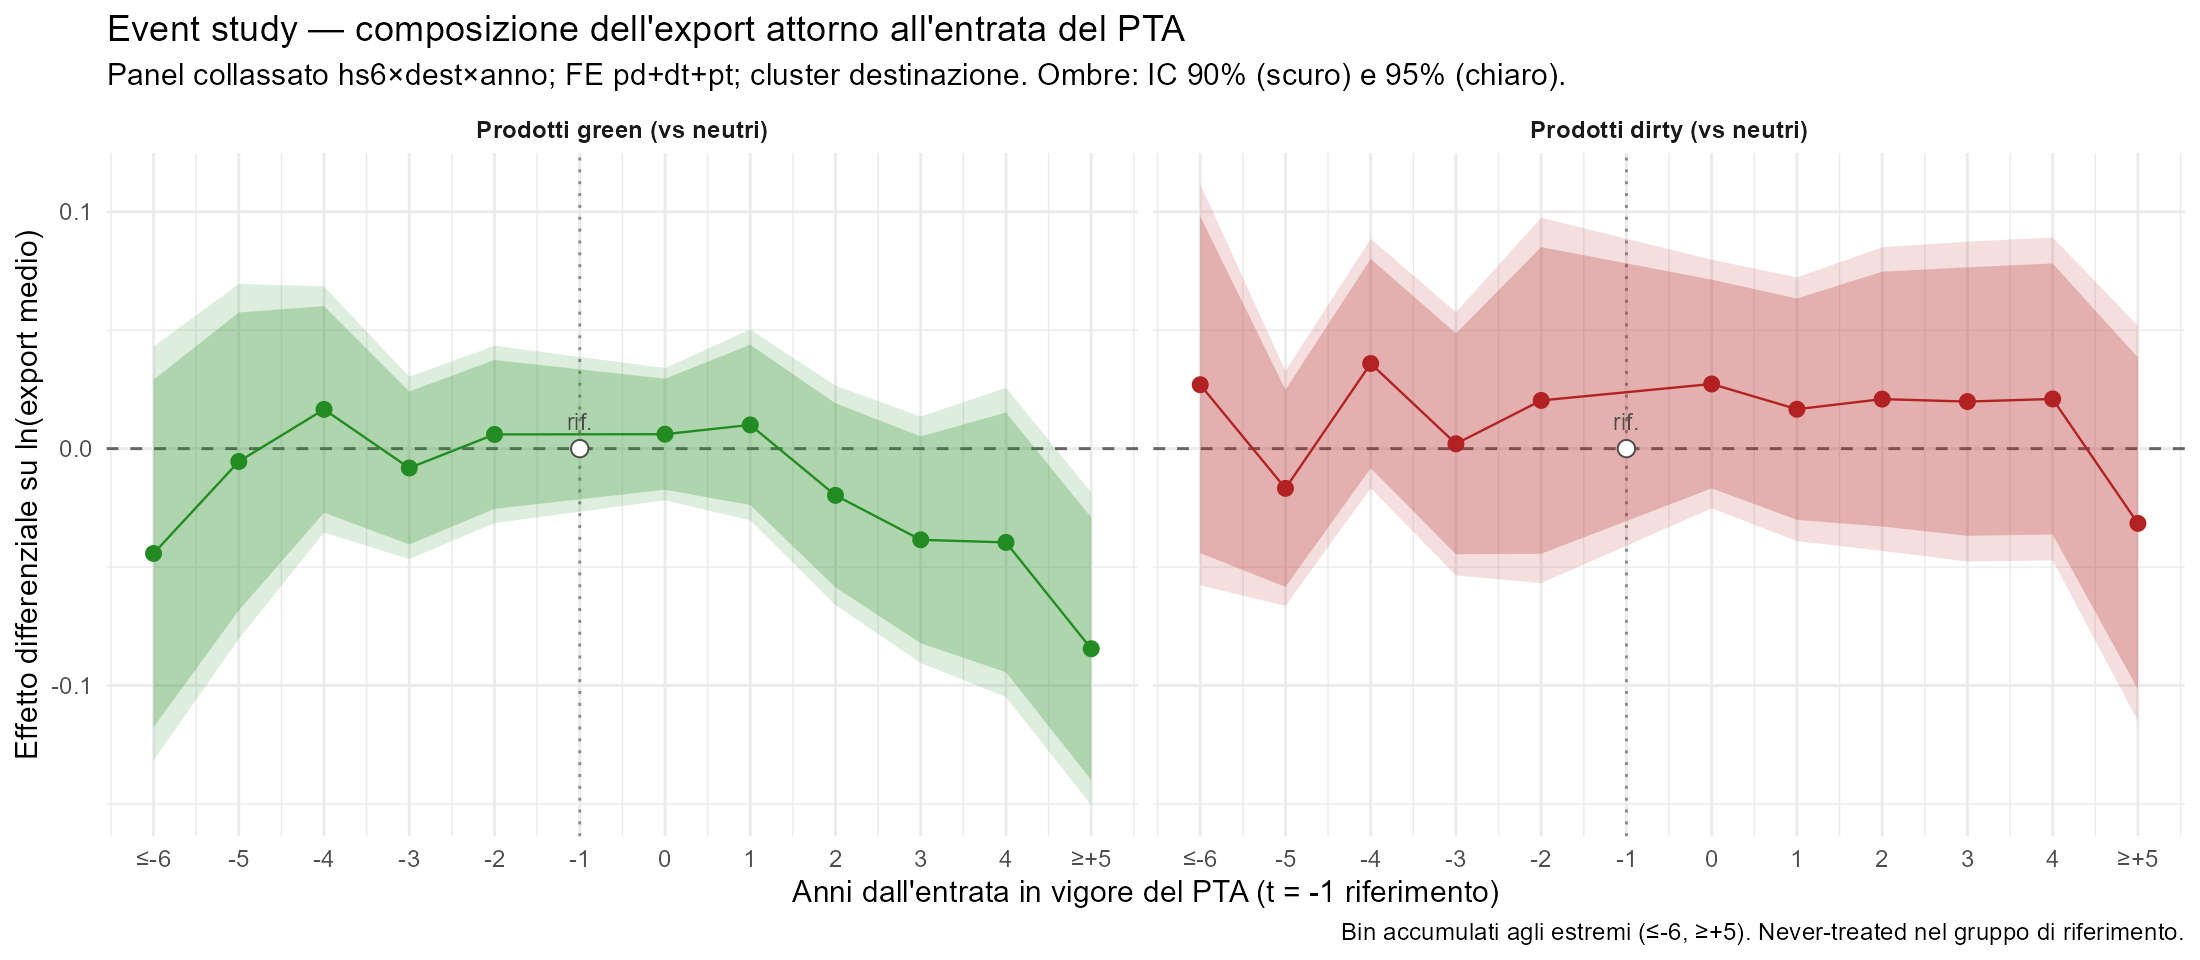
\includegraphics[width=\textwidth]{figures/eventstudy_collapsed_v2.png}
\caption{Event study: green and dirty vs.\ neutral products around PTA entry into
force. Collapsed panel; FE $pd + dt + pt$; destination-clustered 95\% confidence bands;
$t = -1$ is the reference period; endpoint bins accumulate.}
\label{fig:es}
\end{figure}

A mild negative drift for green products in the late post-period (bins $\geq +5$) is
identified only by early cohorts (ASEAN 2005, Chile 2006, Pakistan 2007, New Zealand
2008). It disappears under the Sun--Abraham estimator applied to the destination-level
composition gap: the aggregated ATT is $-0.042$ ($p = 0.27$) for the green gap and
$+0.073$ ($p = 0.28$) for the dirty gap --- consistent with early-cohort heterogeneity
rather than any effect of treatment \citep{sun2021}. The Sun--Abraham estimator answers a
narrower question than equation~\eqref{eq:main} --- it binarizes treatment (EP present or
absent, discarding depth), carries no depth control, and operates on a destination--year
composition gap collapsed across products --- so it should not be read as a replication.
It is a diagnostic for staggered-timing and cohort heterogeneity, and that is how it is
used here.

The full interaction-weighted event study is reported in Appendix~\ref{app:sunab}. With
the standard errors produced by \texttt{eventstudyinteract} --- which, unlike
\texttt{fixest::sunab}, accounts for the uncertainty in the estimated cohort shares used
as weights --- no coefficient in the $[-10, +8]$ window is individually distinguishable
from zero on either margin. Two or three nominally significant coefficients appear among
28 estimates, which is what sampling noise produces under exactly flat pre-trends with 23
treated clusters. The ATT is null across all three specification variants: $p = 0.28$ in
the baseline, $p = 0.11$ in the $[-6, +5]$ window, $p = 0.30$ excluding the 2014--2015
cohorts.

\subsection{The dirty margin: anatomy of a false positive}\label{sec:dirty}

The WB$\times$dirty coefficient in the collapsed panel ($-0.0119$, asymptotic $p < 0.001$)
warrants a subsection of its own. It illustrates, step by step, how a coefficient that
looks robust under standard inference falls apart under scrutiny.

The wild cluster bootstrap raises the $p$-value to 0.07. Permutation inference on the
exact estimating equation goes further: reshuffling entire EP profiles across the 23
treated destinations, 27.7\% of placebo draws produce a coefficient as large in absolute
value, giving $p = 0.28$. A coarser permutation on a destination--year--product-type
aggregate reverses the sign entirely ($+0.005$, $p = 0.49$). The aggregation removes the
within-cell heterogeneity across firms and product varieties that the disaggregated
coefficient exploits, so the two tests are not answering exactly the same question, but
they reach the same verdict. Sign instability under aggregation is itself evidence of
fragility.

A leave-one-out exercise across the 23 treated destinations reveals the mechanism, and it
is not the one the phrase ``driven by a single country'' usually implies. The
\emph{point estimate} is remarkably stable: it sits between $-0.0097$ and $-0.0133$ in
every one of the 23 leave-one-out samples. Dropping large treated destinations such as
India or Pakistan moves it by 1 to 4\% while leaving the standard error essentially
unchanged. Those are not the pivotal observations.

What is not stable is the \emph{precision}. Dropping Australia moves the coefficient by
13\% (to $-0.0103$) but nearly triples its standard error, from 0.0030 to 0.0087: it is
this, not the movement of the estimate, that carries the $p$-value to 0.24. Dropping
South Korea doubles the standard error, giving $-0.0097$ with $p = 0.09$. Australia and
South Korea are therefore not outliers exerting leverage on the estimate. They supply the
variation that identifies it, and removing them leaves the design without enough
information to speak --- rather than with a different answer. The right description is
that the coefficient is identified by a thin slice of variation concentrated in two
destinations, not that those destinations pull the estimate in the wrong direction.

The exercise with the DESTA depth control makes the point sharper. With TotalDepth,
Australia is the pivotal destination; with DESTA, Australia's exclusion leaves the
coefficient at $-0.0110$ with $p = 0.001$, and it is South Korea whose removal triples
the standard error and gives $p = 0.14$. Which destination the precision depends on is
itself a function of a modelling choice that has nothing to do with environmental
content. A genuine identified effect does not behave this way.

The TREND index never shows the effect (bootstrap $p = 0.86$). In the full panel the
coefficient is $-0.0044$ (asymptotic $p = 0.052$); the wild cluster bootstrap raises it
to $p = 0.18$, with a 95\% interval of $[-0.043, +0.011]$. The marginal signal under
asymptotics is erased by robust inference on both panels independently. The honest
reading is that the dirty margin is a false positive of exactly the type few-treated-cluster
designs can manufacture: an estimate that is overwhelming under asymptotic standard errors
and that clears none of the same battery applied to the green margin. It belongs in the
paper as a descriptive pattern and a methodological warning.

\subsection{Provision bundling and the limits of heterogeneity analysis}\label{sec:bundling}

Aggregate EP indices combine provisions with an identifiable trade mechanism and
cooperation language that has none. On any aggregate null, this is the natural objection
--- and it is correct. The response here is not to refute it but to show how extreme the
bundling is, and what that implies for interpretation.

Summing WB\_EP\_Depth across the 25 treated destinations gives 150 provisions checked in
total; 5.3\% fall in \texttt{GreenLiberalization} or \texttt{StandardsNonRegression},
the two sub-indices with a direct trade mechanism. TREND, an independently constructed
and far more granular coding, reaches the same conclusion: of 437 provisions across the
same destinations, \texttt{GreenMarketAccess} is 0.92\%. At the agreement level, TREND's
binding-obligations clause (\texttt{X5.01.01}) appears in exactly one of the 14--15
Chinese agreements in the database (China--Korea, 2015). Table~\ref{tab:mechanism} puts
both codings side by side.

\begin{table}[htbp]
\centering
\caption{Trade-mechanism content as a share of total checked provisions}
\label{tab:mechanism}
\small
\begin{threeparttable}
\begin{tabular}{lccc}
\toprule
 & Total checked & Trade-mechanism provisions & Share \\
\midrule
WB (\texttt{GreenLiberalization} + \texttt{StandardsNonRegression}) & 150 & 8 & 5.3\% \\
TREND (\texttt{GreenMarketAccess}) & 437 & 4 & 0.92\% \\
\midrule
 & Agreements & With binding clause & \\
\midrule
TREND (\texttt{X5.01.01} Binding obligations) & 14--15 & 1 (China--Korea, 2015) & 6.7\% \\
\bottomrule
\end{tabular}
\begin{tablenotes}\footnotesize
\item ``Total checked'' sums the relevant depth index across the 25 treated destinations
at each destination's maximum (post-entry) value. Source:
\texttt{Data/Merged/Merged\_TREND\_WB\_Indices\_Only.csv}.
\end{tablenotes}
\end{threeparttable}
\end{table}

The structural consequence is stark. Across the 223 treated destination--years in the
estimation sample, the two WB sub-indices with a direct mechanism are \emph{perfectly}
collinear ($\rho = 1.000$) and non-zero in only three country--years: Korea from 2015
and Switzerland from 2014, always in the same 1:3 proportion. Their interaction terms
therefore load identically in the regression (identical $t$-statistics; coefficients in
exact 3:1 ratio), and the VIF is unbounded. Contrast this with \citet{brandi2020}, who
report a maximum VIF of 4.6 across provision-type variables on their 680-agreement panel:
enough agreements with enough variation in provision type to separately identify the
mechanism sub-components. With 14 agreements, this design cannot.

A reading rule applies to everything that follows: each sub-index replaces the aggregate
index one at a time and is estimated on its own. The resulting coefficients are not
partial effects holding other clause types constant; they absorb whatever variation in
correlated sub-indices moves with each one. This is the only feasible approach, but it
means the table is a set of separate comparisons, not an additive decomposition of the
aggregate index.

What can be said: the mechanism-bearing bundle shows the same pattern as the aggregate.
Green never responds (WB \texttt{GreenLiberalization}$\times$green: $p = 0.90$; TREND
\texttt{GreenMarketAccess}$\times$green: $p = 0.38$). The dirty interaction is marginally
negative on asymptotic $p$-values ($p = 0.04$--$0.07$), but this is the same
asymptotics-only signal documented in Section~\ref{sec:dirty}, which does not survive
robust inference.

The placebo sub-indices (without a trade mechanism) are more interesting and worth
reporting carefully. TREND soft provisions show nothing on either margin ($\times$green:
$p = 0.27$; $\times$dirty: $p = 0.86$), consistent with the logic of the null. Regulatory
space clauses do not: they carry $+0.024$ on green and $+0.023$ on dirty, and both survive
the wild cluster bootstrap ($p = 0.046$ and $p = 0.022$, $B = 9{,}999$). This is the only
place in the paper where a sub-index without a trade mechanism registers a signal that
robust inference sustains.

Two features bound what can be read into it, and together they leave the conclusion weak.
First, the two margins move in tandem: the green--dirty differential is $+0.0017$ with
$p = 0.80$, meaning the coefficient describes green and dirty exports rising by the same
amount against the neutral baseline --- not a shift in composition toward cleaner goods.
Second, and more fundamentally, the regulatory-space sub-index is not a clean placebo.
It accounts for 71.5\% of the TREND count across treated destination--years and
correlates 0.90 with TotalDepth; in this specification the depth control flips to
significantly negative ($\times$green: $-0.0011$, $p = 0.006$). Two regressors correlated
at 0.90 splitting into a large positive and a large negative is the same bundling problem
applied to the placebo, not a cleanly identified channel. The defensible conclusion is the
weaker one: this design cannot separate a regulatory-space effect from general agreement
depth, so neither the positive signal nor its absence can serve as a clean falsification
test.

Enforcement provisions (dispute-settlement mechanisms attached to the environmental
chapter) are null on both margins and both codings: WB $\times$green $p = 0.91$, $\times$dirty
$p = 0.90$; TREND $\times$green $p = 0.78$, $\times$dirty $p = 0.71$.

This bundling result reconciles the null with \citet{brandi2020}. Their finding is not
that environmental provisions generically matter; it is driven by the subset of agreements
with explicitly liberalizing or restrictive clauses, identified separately because 680
agreements supply enough cross-agreement variation in provision type. The Chinese PTAs of
this period are, on the same coding, overwhelmingly cooperation-only: mechanism-bearing
content appears in two of the fourteen agreements and is perfectly collinear between its
two components in-sample. A null on the aggregate index is what Brandi et al.'s own
heterogeneity would predict for a sample of this composition. The two results are
complementary. A second compounding difference concerns aggregation: \citet{brandi2020}
work with exporter--importer--year flows, where a composition effect can arise from the
entry or exit of firms or products. The specification here saturates
firm$\times$destination$\times$year fixed effects and identifies from reallocation
\emph{within} the same firm across products --- a strictly more demanding test of the
same hypothesis.

\subsection{Extensive margin}

Log-linear estimates condition on positive flows. If EPs create new green trade at the
extensive margin, intensive estimates miss it \citep{santossilva2006}. On a zero-filled
HS6--destination--year grid (8.2 million cells), PPML estimates confirm the null:
EP$\times$green is $+0.0015$ ($p = 0.74$, WB) and $+0.0001$ ($p = 0.95$, TREND);
EP$\times$dirty is $-0.030$ ($p = 0.06$, WB) and $+0.003$ ($p = 0.55$, TREND). No
green trade creation at the extensive margin; the dirty coefficient is at most marginally
significant and consistent with the non-result reading of Section~\ref{sec:dirty}.

One limitation bears noting: this grid detects green products newly exported to a
destination, but not a new firm beginning to export a product that other Chinese firms
already ship there, which is a common form of firm-level entry. The extensive margin is
probed, not exhausted.

\subsection{Within-firm share: a descriptive complement}

On the firm--destination--year panel of green export shares (13.3 million observations;
FE: firm--destination and year; destination-clustered), the coefficient on WB EP depth
is $-0.0001$ ($p = 0.50$) and on TREND $-0.00006$ ($p = 0.043$, asymptotic). Both are
economically negligible: a one-standard-deviation increase in the TREND count moves the
within-firm green share by three hundredths of a percentage point, and the marginal
asymptotic significance carries the same few-cluster caveat as the rest.

This module is reported as a descriptive complement, not identifying evidence. The
specification regresses the green share on the \emph{level} of EP depth with
firm--destination and year fixed effects --- it does not include firm--destination--year
absorption and therefore inherits the collinearity with the agreement that
Section~\ref{sec:strategy} argues is fatal to any level specification in this setting. A
null from an unidentified specification says nothing in either direction. What the module
establishes, and what is worth having, is that the within-firm green share is flat in the
raw conditional means, which is at least consistent with the composition null.

\subsection{How much the depth control matters}

Environmental depth and general agreement depth correlate at 0.96 within destination and
year. Table~\ref{tab:depthbounds} varies the depth control across four alternatives: none,
aggregate TotalDepth (17 areas), a version restricted to the 14 non-environmental areas
most correlated with EP content, and the independently coded DESTA index \citep{dur2014}.

\begin{table}[htbp]
\centering
\caption{EP$\times$green under alternative depth controls (collapsed panel, WB index)}
\label{tab:depthbounds}
\small
\begin{threeparttable}
\begin{tabular}{lcc}
\toprule
Depth control & EP$\times$green & 95\% CI \\
\midrule
None & $-0.0057$ & $[-0.0118,\ +0.0003]$ \\
\texttt{TotalDepth} aggregate (17 areas) --- \emph{main specification} & $-0.0046$ & $[-0.0182,\ +0.0091]$ \\
\texttt{TotalDepth} targeted (14 areas) & $-0.0033$ & $[-0.0188,\ +0.0123]$ \\
DESTA index (independent source) & $-0.0043$ & $[-0.0129,\ +0.0042]$ \\
\bottomrule
\end{tabular}
\begin{tablenotes}\footnotesize
\item Collapsed panel, fixed effects $pd+dt+pt$, weighted by cell size, destination-clustered.
Asymptotic intervals. The targeted control drops the three WB areas that do not correlate
with EP depth (labour-market regulation, which has zero variance in Chinese agreements;
visa and asylum; subsidies). DESTA covers seven policy areas coded independently of the
World Bank instrument and excludes environmental provisions by construction, which is why
it lowers the VIF from 5.7 to 1.9.
\end{tablenotes}
\end{threeparttable}

\end{table}

The point estimate moves within a band of 0.0024 log points --- narrower than a single
standard error --- stays negative throughout, and every interval contains zero. Dropping
the depth control altogether moves the coefficient away from zero rather than toward it.
The green null does not rest on the choice of depth control.

\subsection{Environmental share of agreement content}

The main specification estimates the marginal effect of one additional provision.
\citet{abman2024} pose a different question: given that an agreement exists, does a more
environmentally weighted agreement move composition? That framing requires restricting to
partner destinations and replacing EP depth with its share of total depth,
$EP_{dt}/TD_{dt}$. On the collapsed panel restricted to the 23 partner destinations
(534{,}846 cells, 516{,}684 surviving singleton removal; the share takes 12 distinct values
in $[0.012, 0.068]$; coefficient of variation 0.19 versus 0.62 for the level), the green
interaction is $-2.25$ (s.e.\ 1.15, $p = 0.06$) and the dirty interaction $-1.60$
(s.e.\ 1.55, $p = 0.32$). The share varies far less than the level, so the standard
errors are correspondingly wide; the green coefficient clears neither conventional
threshold. It is reported because the contrast is the one used by the closest antecedent
in the literature, and because a marginally negative coefficient is the opposite of what
green trade creation would predict --- not because this design identifies it well.

\subsection{Sample robustness}

Table~\ref{tab:robust} collects the full-panel variations. Adding controls (MFN tariff,
market concentration, antidumping exposure) moves the green coefficient to an exact zero
($-0.0002$, $p = 0.94$). Excluding the eleven ASEAN destinations --- the largest single
cohort --- leaves it at $-0.0025$ ($p = 0.48$). Re-including Hong Kong and Macao gives
$-0.0009$ ($p = 0.80$). Across every variation, the dirty coefficient sits between
$-0.0040$ and $-0.0060$ with asymptotic $p$-values of 0.02--0.09: persistently marginal
under asymptotics, robust to none of the same battery applied to the green margin.

\begin{table}[htbp]
\centering
\caption{Sample robustness (full firm-level panel, WB index)}
\label{tab:robust}
\small
\begin{threeparttable}
\begin{tabular}{lcccc}
\toprule
Variation & Obs. & EP$\times$green ($p$) & EP$\times$dirty ($p$) \\
\midrule
Baseline & 21.5M & $-0.0023$ (0.57) & $-0.0044$ (0.052) \\
With controls & 19.3M & $-0.0002$ (0.94) & $-0.0060$ (0.022) \\
Excluding ASEAN & 19.2M & $-0.0025$ (0.48) & $-0.0044$ (0.051) \\
Including HK--Macao & 23.6M & $-0.0009$ (0.80) & $-0.0041$ (0.094) \\
Common support & 21.5M & $-0.0022$ (0.57) & $-0.0044$ (0.052) \\
\midrule
PPML, zero-filled grid & 7.9M cells & $+0.0015$ (0.74) & $-0.0301$ (0.06) \\
Within-firm green share & 13.3M & \multicolumn{2}{c}{$-0.0001$ (0.50)} \\
\bottomrule
\end{tabular}
\begin{tablenotes}\footnotesize
\item Asymptotic destination-clustered p-values in parentheses; the dirty column's
marginal significance does not survive wild cluster bootstrap, permutation, or
leave-one-out inference (Section~\ref{sec:dirty}). Controls: ln(1+MFN tariff), ln HHI,
antidumping indicator.
\end{tablenotes}
\end{threeparttable}

\end{table}

On the tariff control: the variable is the applied duty recorded in the customs data,
not a rate constructed here; it varies across destinations for the same HS6--year in
97.9\% of product--year cells and is therefore a destination-facing tariff, not a
Chinese import duty. Its mean does not fall after PTA entry for partner destinations,
which indicates it is the MFN rather than the preferential rate. The preferential rate
was not obtainable. The headline estimates do not depend on the tariff (it appears only
in the ``with controls'' row and in the CEM matching), and whatever liberalization the
agreements delivered varies at the destination--year level and is absorbed by
$\theta_{fdt}$. The residual threat runs in the conservative direction: if PTA tariff
cuts fell more on green goods, the omitted preferential margin would load onto
EP$\times$green with a positive sign. The estimate is zero.

\subsection{Destination-specific trends}

The central falsification test asks whether allowing each destination its own linear
trend in the green (and dirty) gap changes the conclusion, given that the conservative-bias
argument of Section~\ref{sec:strategy} implies those trends might be correlated with EP
depth. Two variants bracket the answer, estimated on the collapsed panel.

The first adds destination-specific linear trends interacted with green and dirty status
over the full sample period. WB results are essentially unchanged (EP$\times$green
$-0.0051$, bootstrap $p = 0.50$; EP$\times$dirty $-0.0082$, bootstrap $p = 0.28$). The
TREND green interaction flips sign and --- the only instance in the full robustness
battery --- survives the wild cluster bootstrap ($p = 0.012$). Taken at face value it
would say environmental provisions reduce green exports. It should not be taken at face
value. Unit-specific trends estimated over the full sample period absorb post-treatment
dynamics and can reverse the sign of treatment coefficients when effects or cohort
dynamics are present \citep{wolfers2006}; the late negative drift that these trends pick
up is precisely the early-cohort artifact that the Sun--Abraham estimator already
identifies as noise.

The second variant estimates destination-specific slopes on \emph{pre-treatment} years
only and projects them forward before re-estimating the main specification on the
detrended outcome. Every coefficient returns to an imprecise zero: TREND$\times$green
$+0.0074$, bootstrap $p = 0.18$; WB$\times$green $+0.0168$, bootstrap $p = 0.71$; dirty
interactions $p = 0.30$--$0.62$. That the one nominally robust coefficient in the
full-period trend exercise reverses sign entirely depending on how the trends are
estimated identifies it as an artifact of the trend specification. The composition null
stands against destination-specific linear drifts in green demand, the most natural form
of the selection-on-trends confounder.

\subsection{CO$_2$ intensity as a continuous dirty measure}

The binary dirty indicator groups HS6 products into six classic pollution-intensive
sectors. A continuous intensity measure might tell a different story. I construct one
from the replication data of \citet{shapiro2021}, which reports China-specific CO$_2$
emission intensities for 47 EXIOBASE industries. HS6 products are mapped to ISIC3
divisions via the same HS1996--ISIC3 concordance used for the binary classification;
unmatched codes (9.5\% of the panel) are assigned the sample mean. The resulting measure
validates against the existing trichotomy without circularity: mean intensity is 0.0012
for dirty products, 0.0008 for neutral, and 0.0006 for green, monotonic in the expected
direction.

Re-estimating equation~\eqref{eq:main} on the collapsed panel with the standardized
intensity in place of the binary dirty indicator gives EP$\times$intensity $= -0.0025$
(WB, bootstrap $p = 0.71$) and $-0.0013$ (TREND, asymptotic $p = 0.012$, bootstrap
$p = 0.06$). The continuous measure fades under robust inference the same way the binary
one does.

\subsection{Alternative outcomes: quantity, unit value, and trimming}

Log export value conflates shipment volume and price per unit. If EPs redirect
composition without moving average prices --- or vice versa --- the value estimate would
be an artifact of two channels canceling. Table~\ref{tab:outcomes} re-estimates
equation~\eqref{eq:main} on the collapsed panel for three outcome variables: log export
value (the main specification), log export quantity, and log unit value.

\begin{table}[htbp]
\centering
\caption{EP$\times$green and EP$\times$dirty across outcome variables (collapsed panel)}
\label{tab:outcomes}
\small
\begin{threeparttable}
\begin{tabular}{llcccc}
\toprule
 & & \multicolumn{2}{c}{WB index} & \multicolumn{2}{c}{TREND index} \\
\cmidrule(lr){3-4}\cmidrule(lr){5-6}
Outcome & Interaction & Coeff. & Boot.\ $p$ & Coeff. & Boot.\ $p$ \\
\midrule
Log export value   & $\times$green & $-0.0046$ & 0.65 & $-0.0002$ & 0.87 \\
                   & $\times$dirty & $-0.0119$ & 0.07 & $-0.0015$ & 0.86 \\
\addlinespace
Log export quantity & $\times$green & $-0.0055$ & 0.53 & $+0.0019$ & 0.43 \\
                    & $\times$dirty & $-0.0115$ & 0.25 & $-0.0004$ & 0.89 \\
\addlinespace
Log unit value     & $\times$green & \multicolumn{2}{c}{$p \in [0.85, 0.95]$} &
                                     \multicolumn{2}{c}{$p \in [0.85, 0.95]$} \\
                   & $\times$dirty & \multicolumn{2}{c}{$p \in [0.85, 0.95]$} &
                                     \multicolumn{2}{c}{$p = 0.16$ (TREND)} \\
\bottomrule
\end{tabular}
\begin{tablenotes}\footnotesize
\item Collapsed panel; FE $pd + dt + pt$; destination-clustered wild cluster bootstrap
($B = 9{,}999$). Log export value row is the baseline collapsed-panel estimate from
Table~\ref{tab:main}. Unit-value coefficients are small in magnitude and reported as
$p$-value ranges; exact coefficients available from the author. Asymptotic $p$-values
for log unit value are between 0.85 and 0.95 on all four interactions except
TREND$\times$dirty ($p = 0.16$).
\end{tablenotes}
\end{threeparttable}
\end{table}

No outcome registers a significant effect on either index or either product type. The
null is consistent across value, quantity, and price --- it is not an artifact of
channels canceling in the value aggregate.

\paragraph{Trimming.}
Trimming log export value at the 1st and 99th percentiles removes 2.0\% of collapsed-panel
cells (3{,}773{,}498 $\to$ 3{,}698{,}033); after singleton removal the estimation sample is
3{,}605{,}798. The green null is unaffected: EP$\times$green $-0.0048$ (WB, bootstrap
$p = 0.61$) and $+0.0018$ (TREND, bootstrap $p = 0.41$). The dirty margin reproduces
its characteristic pattern --- marginally significant under WB ($p = 0.041$), null under
TREND ($p = 0.89$) --- consistent with a false positive rather than a genuine effect.

% ============================================================================
\section{Conclusion}\label{sec:conclusion}
% ============================================================================

China's trade agreements did not shift the composition of its exports between 2000 and 2015.
On the green margin, the finding is a \emph{bounded null}: stable across six estimation
designs and nine sample variations, robust to bootstrap and permutation inference, and
bounded from above by roughly one quarter of the reference estimate in the aggregate
literature. This is not a failure to reject. It is a precisely circumscribed statement
about the absence of a specific effect --- the kind the literature has documented elsewhere
under different conditions.

On the dirty margin, the finding is a \emph{non-result}. A coefficient that is overwhelming
under asymptotic standard errors survives none of the inference battery applied to the green
margin. The leave-one-out exercise reveals why: the point estimate is stable across all 23
exclusions ($-0.0097$ to $-0.0133$), but the standard error nearly triples when either of
two destinations is dropped. Precision, not the estimate, is what two specific destinations
supply. An identified effect does not behave this way.

The central reading is about content. Environmental provisions affect trade when they are
specific, binding, and targeted at a product category --- \citet{abman2024} show this for
deforestation, \citet{brandi2020} for trade composition. China's chapters of this period
were thin and cooperation-heavy: the two WB sub-indices with a direct trade mechanism are
perfectly collinear in-sample and appear in only three treated country--years. The policy
implication is direct: a chapter in an agreement is not itself the instrument. What the
chapter contains is.

Methodologically, the paper adds a cautionary case. With treatment concentrated across
roughly a dozen agreements, asymptotically significant composition effects can emerge and
dissolve under honest inference. Bootstrap, permutation, and leave-one-out --- applied not
as robustness appendices but as the primary mode of inference --- should be standard
practice for this class of design.

Three limitations bear noting. The preferential tariff rate was not obtainable; the headline
estimates are independent of it, but the MFN rate used as a control is an imperfect proxy.
A continuous-dose estimator in the spirit of \citet{callaway2024} is not implemented; the
TWFE coefficient is a weighted average of cohort-specific effects, though the permutation
test is agnostic about this weighting. The extensive margin is probed at the
product--destination level: new firm entry into a destination where other Chinese firms
already export the same green product is not captured.

% ============================================================================
\begin{thebibliography}{99}
% ============================================================================

\bibitem[Abadie et al.(2023)]{abadie2023}
Abadie, A., Athey, S., Imbens, G.~W., \& Wooldridge, J.~M. (2023).
When should you adjust standard errors for clustering?
\textit{Quarterly Journal of Economics}, 138(1), 1--35.

\bibitem[Abman et al.(2024)]{abman2024}
Abman, R., Lundberg, C., \& Ruta, M. (2024).
The effectiveness of environmental provisions in regional trade agreements.
\textit{Journal of International Economics}, 148, 103875.

\bibitem[Baccini et al.(2017)]{baccini2017}
Baccini, L., Pinto, P.~M., \& Weymouth, S. (2017).
The distributional consequences of preferential trade liberalization: Firm-level evidence.
\textit{World Politics}, 69(2), 373--408.

\bibitem[Baghdadi et al.(2013)]{baghdadi2013}
Baghdadi, L., Martinez-Zarzoso, I., \& Zitouna, H. (2013).
Are RTA agreements with environmental provisions reducing emissions?
\textit{Journal of International Economics}, 90(2), 378--390.

\bibitem[Bertrand et al.(2004)]{bertrand2004}
Bertrand, M., Duflo, E., \& Mullainathan, S. (2004).
How much should we trust differences-in-differences estimates?
\textit{Quarterly Journal of Economics}, 119(1), 249--275.

\bibitem[Callaway et al.(2021)]{callaway2021}
Callaway, B., \& Sant'Anna, P.~H.~C. (2021).
Difference-in-differences with multiple time periods.
\textit{Journal of Econometrics}, 225(2), 200--230.

\bibitem[Callaway et al.(2024)]{callaway2024}
Callaway, B., Goodman-Bacon, A., \& Sant'Anna, P.~H.~C. (2024).
Difference-in-differences with a continuous treatment.
\textit{NBER Working Paper} 32117.

\bibitem[Cameron et al.(2008)]{cameron2008}
Cameron, A.~C., Gelbach, J.~B., \& Miller, D.~L. (2008).
Bootstrap-based improvements for inference with clustered errors.
\textit{Review of Economics and Statistics}, 90(3), 414--427.

\bibitem[Cherniwchan(2017)]{cherniwchan2017}
Cherniwchan, J. (2017).
Trade liberalization and the environment: Evidence from NAFTA and US manufacturing.
\textit{Journal of International Economics}, 105, 130--149.

\bibitem[Conley \& Taber(2011)]{conley2011}
Conley, T.~G., \& Taber, C.~R. (2011).
Inference with ``difference in differences'' with a small number of policy changes.
\textit{Review of Economics and Statistics}, 93(1), 113--125.

\bibitem[Copeland et al.(2022)]{copeland2022}
Copeland, B.~R., Shapiro, J.~S., \& Taylor, M.~S. (2022).
Globalization and the environment.
In G.~Gopinath, E.~Helpman, \& K.~Rogoff (Eds.), \textit{Handbook of International
Economics} (Vol.\ 5). Elsevier.

\bibitem[Correia et al.(2017)]{correia2017}
Correia, S., Guimarães, P., \& Zylkin, T. (2021).
Fast Poisson estimation with high-dimensional fixed effects.
\textit{Stata Journal}, 21(4), 1038--1072.

\bibitem[de Chaisemartin \& D'Haultfœuille(2020)]{dechaisemartin2020}
de Chaisemartin, C., \& D'Haultfœuille, X. (2020).
Two-way fixed effects estimators with heterogeneous treatment effects.
\textit{American Economic Review}, 110(9), 2964--2996.

\bibitem[Dechezleprêtre \& Sato(2017)]{dechezlepretre2017}
Dechezleprêtre, A., \& Sato, M. (2017).
The impacts of environmental regulations on competitiveness.
\textit{Review of Environmental Economics and Policy}, 11(2), 183--206.

\bibitem[Brandi et al.(2020)]{brandi2020}
Brandi, C., Schwab, J., Berger, A., \& Morin, J.~F. (2020).
Do environmental provisions in trade agreements make exports from developing countries
greener?
\textit{World Development}, 129, 104899.

\bibitem[Dür et al.(2014)]{dur2014}
Dür, A., Baccini, L., \& Elsig, M. (2014).
The design of international trade agreements: Introducing a new dataset.
\textit{Review of International Organizations}, 9(3), 353--375.

\bibitem[Eckel \& Neary(2010)]{eckel2010}
Eckel, C., \& Neary, J.~P. (2010).
Multi-product firms and flexible manufacturing in the global economy.
\textit{Review of Economic Studies}, 77(1), 188--217.

\bibitem[Feenstra \& Hanson(2004)]{feenstra2004}
Feenstra, R.~C., \& Hanson, G.~H. (2004).
Intermediaries in entrepôt trade: Hong Kong re-exports of Chinese goods.
\textit{Journal of Economics \& Management Strategy}, 13(1), 3--35.

\bibitem[Fischer \& Stöckl(2021)]{fischer2021}
Fischer, S., \& Stöckl, S. (2021).
Wild cluster bootstrap in Stata: Implementation of the fwildclusterboot package.
\textit{Stata Journal}, 21(4).

\bibitem[Fisher(1935)]{fisher1935}
Fisher, R.~A. (1935).
\textit{The Design of Experiments}. Edinburgh: Oliver and Boyd.

\bibitem[Goodman-Bacon(2021)]{goodmanbacon2021}
Goodman-Bacon, A. (2021).
Difference-in-differences with variation in treatment timing.
\textit{Journal of Econometrics}, 225(2), 254--277.

\bibitem[Head \& Mayer(2014)]{headmayer2014}
Head, K., \& Mayer, T. (2014).
Gravity equations: Workhorse, toolkit, and cookbook.
In G.~Gopinath, E.~Helpman, \& K.~Rogoff (Eds.), \textit{Handbook of International
Economics} (Vol.\ 4, pp.\ 131--195). Elsevier.

\bibitem[Hofmann et al.(2017)]{hofmann2017}
Hofmann, C., Osnago, A., \& Ruta, M. (2017).
Horizontal depth: A new database on the content of preferential trade agreements.
\textit{World Bank Policy Research Working Paper} 7981.

\bibitem[Iacus et al.(2012)]{iacus2012}
Iacus, S.~M., King, G., \& Porro, G. (2012).
Causal inference without balance checking: Coarsened exact matching.
\textit{Political Analysis}, 20(1), 1--24.

\bibitem[Larch \& Yotov(2025)]{larch2025}
Larch, M., \& Yotov, Y. (2025).
Estimating gravity with zero trade flows: A practical guide.
\textit{Journal of International Economics}.

\bibitem[Low \& Yeats(1992)]{low1992}
Low, P., \& Yeats, A. (1992).
Do ``dirty'' industries migrate?
\textit{World Bank Discussion Paper} 159.

\bibitem[MacKinnon \& Webb(2017)]{mackinnon2017}
MacKinnon, J.~G., \& Webb, M.~D. (2017).
Wild bootstrap inference for wildly different cluster sizes.
\textit{Journal of Applied Econometrics}, 32(2), 233--254.

\bibitem[Mani \& Wheeler(1998)]{mani1998}
Mani, M., \& Wheeler, D. (1998).
In search of pollution havens? Dirty industry in the world economy, 1960 to 1995.
\textit{Journal of Environment \& Development}, 7(3), 215--247.

\bibitem[Morin et al.(2018)]{morin2018}
Morin, J.~F., Pauwelyn, J., \& Hollway, J. (2018).
The trade regime as a complex adaptive system: Exploration and exploitation of
environmental norms in trade agreements.
\textit{Journal of International Economic Law}, 20(2), 365--390.

\bibitem[Neri \& Santacreu-Vasut(2023)]{neri2023}
Neri, L., \& Santacreu-Vasut, E. (2023).
The heterogeneous effects of deep trade agreements on exports.
\textit{Review of World Economics}, 159(1), 241--277.

\bibitem[Rajan \& Zingales(1998)]{rajan1998}
Rajan, R.~G., \& Zingales, L. (1998).
Financial dependence and growth.
\textit{American Economic Review}, 88(3), 559--586.

\bibitem[Roodman et al.(2019)]{roodman2019}
Roodman, D., Nielsen, M.~Ø., MacKinnon, J.~G., \& Webb, M.~D. (2019).
Fast and wild: Bootstrap inference in Stata using boottest.
\textit{Stata Journal}, 19(1), 4--60.

\bibitem[Santos Silva \& Tenreyro(2006)]{santossilva2006}
Santos Silva, J.~M.~C., \& Tenreyro, S. (2006).
The log of gravity.
\textit{Review of Economics and Statistics}, 88(4), 641--658.

\bibitem[Sauvage(2014)]{sauvage2014}
Sauvage, J. (2014).
The stringency of environmental regulations and trade in environmental goods.
\textit{OECD Trade and Environment Working Paper} 2014/03.

\bibitem[Shapiro(2021)]{shapiro2021}
Shapiro, J.~S. (2021).
The environmental bias of trade policy.
\textit{Quarterly Journal of Economics}, 136(2), 831--886.

\bibitem[Sun \& Abraham(2021)]{sun2021}
Sun, L., \& Abraham, S. (2021).
Estimating dynamic treatment effects in event studies with heterogeneous treatment
effects.
\textit{Journal of Econometrics}, 225(2), 175--199.

\bibitem[Wolfers(2006)]{wolfers2006}
Wolfers, J. (2006).
Did unilateral divorce laws raise divorce rates? A reconciliation and new results.
\textit{American Economic Review}, 96(5), 1802--1820.

\end{thebibliography}

% ============================================================================
\appendix
% ============================================================================

\section{Equivalence of the collapsed and firm-level panels}\label{app:pddt}

The collapsed panel aggregates firm--HS6--destination--year observations to
HS6--destination--year cells with outcome equal to the within-cell mean of log exports
and weights equal to cell counts. Under fixed effects $pd + dt + pt$ the weighted
cell-level regression is algebraically identical to the unweighted micro-level regression
under the same fixed effects. Verification to seven significant figures: the
EP$\times$green coefficient is $-0.0045685$ in both; the EP$\times$dirty coefficient is
$-0.011873$ in both. The result is exact up to floating-point precision and holds by
construction of the collapse and weights, not by approximation.

\section{Saturation ladder}\label{app:ladder}

Table~\ref{tab:ladder} reports EP-depth coefficients on log exports across twelve
fixed-effects structures, from the sparsest (product--destination and year) to the most
saturated (adding firm--destination--year and product--year). Moving from left to right,
the coefficient falls monotonically, reaching a precise zero in the three most saturated
structures. This is the empirical documentation of the collinearity argument of
Section~\ref{sec:strategy}: the pattern is the signature of selection, not treatment.

\begin{table}[htbp]
\centering
\footnotesize
\caption{Perch\'e l'effetto \emph{di livello} non \`e stimabile: la scala di saturazione}
\label{tab:ladder}
\begin{threeparttable}
{
\def\sym#1{\ifmmode^{#1}\else\(^{#1}\)\fi}
\begin{tabular}{lcccc}
\toprule
 & \multicolumn{2}{c}{\textit{WB EP Depth}} & \multicolumn{2}{c}{\textit{TREND EP Count}} \\
\cmidrule(lr){2-3}\cmidrule(lr){4-5}
Fixed Effects & (1) Baseline & (2) Controls & (3) Baseline & (4) Controls \\
\midrule
\textit{fpd} + \textit{t} & 0.00311 & 0.00354 & 0.00040 & 0.00046 \\
 & (0.00251) & (0.00260) & (0.00047) & (0.00048) \\
\addlinespace
\textit{fpt} + \textit{pd} & 0.00463\sym{*} & 0.00476\sym{*} & 0.00101\sym{**} & 0.00105\sym{**} \\
 & (0.00270) & (0.00274) & (0.00051) & (0.00052) \\
\addlinespace
\textit{fpt} + \textit{fpd} & 0.00010 & 0.00010 & 0.00016 & 0.00016 \\
 & (0.00326) & (0.00329) & (0.00061) & (0.00060) \\
\addlinespace
\textit{fpd} + \textit{pt} & 0.00087 & 0.00103 & 0.00028 & 0.00030 \\
 & (0.00225) & (0.00221) & (0.00044) & (0.00044) \\
\midrule
\multicolumn{5}{l}{\footnotesize \textit{Notes}: SEs clustered at destination (\texttt{country\_code}). N varies across specs.} \\
\multicolumn{5}{l}{\footnotesize \sym{*} \(p<0.10\), \sym{**} \(p<0.05\), \sym{***} \(p<0.01\)} \\
\bottomrule
\end{tabular}
}
\begin{tablenotes}[flushleft]\footnotesize
\item Variabile dipendente: logaritmo del valore esportato. Ogni riga aggiunge effetti fissi pi\`u stringenti, cio\`e elimina confronti sempre meno credibili.
\item Notazione: \textit{f} = impresa, \textit{p} = prodotto, \textit{d} = destinazione, \textit{t} = anno.
\item Il coefficiente \`e piccolo ovunque e la significativit\`a compare solo nella specificazione intermedia, per poi sparire quando si satura. \`E il segno tipico della \emph{selezione}: la Cina firma accordi con i partner verso cui gi\`a esporta molto. Da qui la scelta di abbandonare l'effetto di livello e passare alla composizione.
\item Errore standard fra parentesi, raggruppato per destinazione.
\end{tablenotes}
\end{threeparttable}
\end{table}


\section{Sun--Abraham event study}\label{app:sunab}

Figure~\ref{fig:sunab} and Table~\ref{tab:sunab} report the interaction-weighted
\citep{sun2021} event study of the green and dirty versus neutral differential, estimated
on the destination-year composition gap and run with \texttt{eventstudyinteract} in
\textsc{Stata}.

A note on standard errors. The cohort shares with which \texttt{eventstudyinteract}
aggregates group-specific effects are themselves estimated from the data; Sun and Abraham
(2021) prescribe including that estimation uncertainty in the variance.
\texttt{eventstudyinteract} does so; \texttt{fixest::sunab} in \textsc{R} treats the
shares as fixed weights. The two implementations agree on coefficients to 15 significant
figures but disagree on standard errors. The degree of disagreement is informative: where
a single cohort identifies a period (so there are no shares to estimate), the ratio of
the two standard errors is exactly 1.00; where many cohorts contribute and their effects
are heterogeneous, the ratio reaches 3 to 4. The standard errors reported here are the
\textsc{Stata} ones, which reflect the full estimation uncertainty.

With these standard errors, no coefficient in the $[-10, +8]$ window is individually
distinguishable from zero on the green or dirty margin. The ATT is $-0.042$ ($p = 0.27$)
for the green gap and $+0.073$ ($p = 0.28$) for the dirty gap. Any apparent pre-trend in
the \textsc{R} output (the lead at $t = -6$ had $p = 0.001$ under \texttt{fixest::sunab})
reflects the treatment of cohort-share uncertainty, not a genuine pre-trend anomaly.

\begin{figure}[htbp]
\centering

\includegraphics[width=\textwidth]{figures/eventstudy_sunab.png}
\caption{Sun--Abraham interaction-weighted event study: green and dirty vs.\ neutral
gap at the destination--year level. 95\% confidence bands based on
\texttt{eventstudyinteract} standard errors, which account for estimation uncertainty
in cohort shares. Endpoint bins at $t \leq -10$ and $t \geq +8$.}
\label{fig:sunab}
\end{figure}

\begin{table}[htbp]
\centering
\footnotesize
\caption{Stimatore di Sun e Abraham applicato al divario di composizione}
\label{tab:sunab}
\begin{threeparttable}
\begin{tabular}{rcccc}
\toprule
Anni dall' & \multicolumn{2}{c}{Divario verdi $-$ neutri} & \multicolumn{2}{c}{Divario sporchi $-$ neutri} \\
\cmidrule(lr){2-3}\cmidrule(lr){4-5}
entrata & Coefficiente & $p$-value & Coefficiente & $p$-value \\
\midrule
-10 & -0.0500$^{**}$ & 0.012 & -0.0356 & 0.356 \\
-9 & -0.0128 & 0.579 & 0.0641$^{*}$ & 0.058 \\
-8 & -0.0001 & 0.997 & -0.0478 & 0.107 \\
-7 & -0.0392$^{**}$ & 0.021 & -0.0186 & 0.362 \\
-6 & 0.0027 & 0.873 & 0.0466$^{***}$ & 0.001 \\
-5 & 0.0022 & 0.938 & -0.0447 & 0.215 \\
-4 & 0.0345 & 0.208 & -0.0210 & 0.445 \\
-3 & 0.0021 & 0.906 & -0.0451$^{*}$ & 0.066 \\
-2 & 0.0034 & 0.820 & -0.0080 & 0.695 \\
+0 & 0.0116 & 0.417 & 0.0579$^{*}$ & 0.056 \\
+1 & 0.0191 & 0.427 & 0.0661 & 0.156 \\
+2 & -0.0049 & 0.863 & 0.0765 & 0.206 \\
+3 & -0.0244 & 0.372 & 0.0921 & 0.119 \\
+4 & -0.0187 & 0.571 & 0.0906 & 0.140 \\
+5 & -0.0233 & 0.537 & 0.1153$^{*}$ & 0.085 \\
+6 & 0.0027 & 0.949 & 0.1264 & 0.108 \\
+7 & -0.0320 & 0.428 & 0.1083 & 0.177 \\
+8 & -0.0779 & 0.113 & 0.0983 & 0.203 \\
\bottomrule
\end{tabular}
\begin{tablenotes}[flushleft]\footnotesize
\item Variante baseline. Finestra mostrata: da $-10$ a $+8$ anni; il file completo copre un intervallo pi\`u ampio.
\item \textbf{Perch\'e serve.} Quando gli accordi entrano in vigore in anni diversi (qui: dal 2002 al 2015), lo stimatore tradizionale pu\`o confondere l'effetto vero con il confronto fra chi \`e stato trattato prima e chi dopo. Sun e Abraham (2021) propongono una correzione che calcola l'effetto separatamente per ogni gruppo di ingresso e poi lo aggrega.
\item \textbf{Come si legge.} La variabile dipendente qui non \`e l'export ma il \emph{divario}: media dei prodotti verdi meno media dei neutri, nella stessa destinazione e anno. Cos\`i il disegno diventa un confronto scaglionato ordinario, a cui il metodo si applica direttamente.
\item Un coefficiente significativo \emph{prima} dell'anno zero \`e un segnale di allarme, non un risultato: va discusso apertamente.
\item $^{*}$ $p<0.10$, $^{**}$ $p<0.05$, $^{***}$ $p<0.01$.
\end{tablenotes}
\end{threeparttable}
\end{table}


\section{Sub-index estimates}\label{app:subindices}

Table~\ref{tab:subindices} reports triple-difference estimates replacing the aggregate EP
index with each sub-index in turn. Each row is a separate regression; the coefficients
are not partial effects. See Section~\ref{sec:bundling} for interpretation.

\begin{table}[htbp]
\centering
\footnotesize
\caption{Scomposizione per tipo di disposizione: quali clausole avrebbero un meccanismo commerciale?}
\label{tab:subindices}
\begin{threeparttable}
\begin{tabular}{lcc}
\toprule
Sotto-indice & $\times$ Verde & $\times$ Sporco \\
\midrule
Liberalizzazione dei beni verdi (WB) & -0.0115 & -0.0876$^{*}$ \\
 & (0.0879) & (0.0483) \\
 & [0.896] & [0.071] \\
\addlinespace
Accesso al mercato per i beni verdi (TREND) & -0.0271 & -0.0491$^{**}$ \\
 & (0.0303) & (0.0243) \\
 & [0.372] & [0.045] \\
\addlinespace
Meccanismo di risoluzione controversie (WB) & -0.0048 & 0.0067 \\
 & (0.0394) & (0.0525) \\
 & [0.903] & [0.898] \\
\addlinespace
Meccanismo di risoluzione controversie (TREND) & 0.0042 & -0.0052 \\
 & (0.0148) & (0.0140) \\
 & [0.778] & [0.709] \\
\addlinespace
Disposizioni vincolanti (TREND) & 0.0022 & -0.0013 \\
 & (0.0047) & (0.0037) \\
 & [0.638] & [0.724] \\
\addlinespace
Disposizioni di sola cooperazione (TREND) & 0.0132 & 0.0019 \\
 & (0.0121) & (0.0108) \\
 & [0.275] & [0.858] \\
\addlinespace
Clausole di spazio regolatorio (TREND) & 0.0242$^{**}$ & 0.0225$^{***}$ \\
 & (0.0099) & (0.0086) \\
 & [0.015] & [0.010] \\
\addlinespace
\midrule
Celle (tutte le righe) & \multicolumn{2}{c}{3,681,023} \\
\bottomrule
\end{tabular}
\begin{tablenotes}[flushleft]\footnotesize
\item Variante baseline, pannello collassato. Ogni riga \`e una stima separata in cui l'indice complessivo \`e sostituito dal sotto-indice indicato; il controllo di profondit\`a resta incluso.
\item \textbf{L'obiezione a cui risponde.} Un indice che somma tutte le disposizioni mescola clausole che potrebbero davvero spostare il commercio (abbassare i dazi sui beni verdi, imporre standard vincolanti) con dichiarazioni di intenti che non hanno alcun meccanismo. Se l'effetto esiste, dovrebbe concentrarsi nelle prime.
\item \textbf{Il limite, che \`e esso stesso un risultato.} Negli accordi cinesi del periodo le disposizioni dotate di un meccanismo commerciale sono rarissime: i due sotto-indici della Banca Mondiale che ne hanno uno sono diversi da zero in soli tre anni-paese e risultano perfettamente sovrapposti fra loro. Non \`e quindi possibile distinguerne gli effetti: non per un difetto del metodo, ma perch\'e quel contenuto negli accordi quasi non c'\`e.
\item Le righe \emph{sola cooperazione} e \emph{spazio regolatorio} funzionano da controllo negativo: sono clausole senza meccanismo commerciale, e l\`i non dovrebbe emergere nulla.
\item Errore standard fra parentesi tonde, $p$-value fra parentesi quadre. $^{*}$ $p<0.10$, $^{**}$ $p<0.05$, $^{***}$ $p<0.01$.
\end{tablenotes}
\end{threeparttable}
\end{table}


\end{document}
